\section{Notre organisation}
%diagrammes de Gant, explication de la méthode de travail
Notre projet s'est déroulé en 3 temps. La première partie a consisté à lire des articles concernant le monoïde plaxique afin de s'approprier les définitions. Une grande partie de ce temps a été passé sur l'article de Brown~\cite{brown2021plactic} pour bien comprendre les différents algorithmes : d'abord la multiplication et ensuite les algorithmes de division. Comme expliqué dans la section \ref{etat_recherche}, la publication de l'article de Monico~\cite{monico2022division} en décembre a changé nos plans. Nous avons pris le temps de bien comprendre ses algorithmes avant de les implémenter. L'implémentation en Rust de la division de Monico a justement constitué la deuxième partie du projet. Cela a d'abord demandé une phase d'apprentissage du langage avant de pouvoir commencer à coder. Enfin, dans un dernier temps, nous avons utilisé le code écrit pour comparer les algorithmes tout en écrivant ce rapport. Vous trouverez ci-dessous notre diagramme de Gant prévisionnel et le diagramme de Gant réel.
\begin{figure}[!h]
	\centering
	
\includegraphics[width=\textwidth]{gant_previsionnel.png}
	\caption{Diagramme de Gant prévisionnel}
\end{figure}
\begin{figure}[!h]
	\centering
	
\includegraphics[width=\textwidth]{gant_reel.png}
	\caption{Diagramme de Gant réel}
\end{figure}

\pagebreak
Tout au long du projet, nous avons régulièrement fait des réunions avec notre tuteur (au début toutes les semaines puis un peu plus espacées ensuite) où nous échangions sur ce que nous avions fait depuis la réunion précédente et définissions les prochains objectifs. Nous faisions à chaque fois un petit compte rendu pour se souvenir de ce qui a été dit. Pour mettre notre code en commun, nous avons utilisé Git et GitLab. Antoine s'est occupé de l'implémentation de la multiplication et des algorithmes de Monico et Aimadeddine des autres algorithmes de division.

Notre code est disponible à l'adresse suivante : \href{https://gitlab.isima.fr/leorober/plactic-monoid}{https://gitlab.isima.fr/leorober/plactic-monoid}. Il se situe dans le dossier \texttt{src} et est séparé en plusieurs fichiers contenants chacun un module. 

\section{Préparation de l'implémentation}
\subsection{Le Rust}
Nous avons effectué toutes nos implémentations en Rust. Ce langage nous a été imposé par notre tuteur. Il s'agit d'un langage récent (la première version stable est sortie en 2015), compilé, multiplateformes avec un typage statique et ayant une syntaxe inspirée du C. Il cherche à corriger les défauts du C tout en gardant un niveau de performances similaire. Pour cela, il apporte de nouvelles fonctionnalités telles que l'inférence de type, la généricité ou encore le filtrage par motif. Il possède une bibliothèque standard qui contient entre autre toutes les structures de données courantes comme les vecteurs ou les chaines de caractères, les opérations sur les types primitifs, des outils pour le multi-theading, etc. Le Rust n'est pas un langage orienté objet mais en possède toutes fois certains aspects. En effet, on peut utiliser des traits qui sont des ensembles de méthodes. Une structure peut implémenter un trait comme un objet implémente une interface en programmation orientée objet.

En Rust, le code est organisé en modules indépendants au sein desquels on regroupe des structures et fonctions, qui peuvent avoir une visibilité publique ou privée. Le langage utilise un système de macros qui permet de faire de la métaprogrammation. Leur nom se termine par un point d'exclamation. Par exemple, l'affichage dans le terminal s'effectue à l'aide de la macro \texttt{println!}. Il est possible d'utiliser des attributs (commençants par \texttt{\#}) qui sont interprétés par le compilateur pour faire de la compilation conditionnelle, désactiver des warnings ou implémenter automatiquement certains traits pour les structures créés. Il existe un attribut permettant de d'informer le compilateur qu'un module est un module de test. Il est ainsi très facile de faire des tests : une commande permet de lancer tous les tests du projet et ils sont ignorés lors de la compilation normale. Rust supporte aussi la génération automatique de documentation en HTML à partir de commentaires écrits en Markdown dans le code. Nous avons utilisé cette fonctionnalité : la doc générée se trouve dans le répértoire \href{https://gitlab.isima.fr/leorober/plactic-monoid/-/tree/master/target/doc/plactic_monoid}{target/doc/plactic\_monoid}

Rust vient avec une gestionnaire de paquets nommé Cargo qui rend simple la gestion des dépendances et la compilation. Lors de la création d'un projet avec Cargo, la structure de dossiers est automatiquement créé est le répertoire git est initialisé. Par défaut, Cargo compile pour le débogage. On peut ajouter une option pour compiler pour le déploiement, le code sera alors optimisé. Pour lancer les tests, on utilise par exemple la commande \texttt{cargo test}.

Mais ce qui fait la particularité de Rust, c'est surtout son système de gestion de la mémoire basé sur les concepts de possession et d'emprunt. À l'ISIMA, nous avons étudié deux façons pour un langage de gérer la mémoire. La première, que l'on retrouve en C/C++, est de laisser au développeur la charge de la gestion de la mémoire. Cette solution est risquée car de nombreux problèmes peuvent apparaîtrent si la mémoire est mal libérée ou si l'on accède à des mauvaises zones mémoires. La seconde, choisie par Java, est d'utiliser un ramasse-miettes. Cela à pour inconvénient de ralentir l'exécution du programme. Rust a fait un choix différent. En Rust, une valeur a toujours un et un seul propriétaire. La valeur peut changer de propriétaire, mais dans ce cas l'ancien propriétaire ne peut plus l'utiliser. La mémoire est automatiquement libérée lorsque le propriétaire sort de la portée où il a été déclaré. Il est possible de créer une référence sur une valeur pour l'emprunter à son propriétaire. Par défaut, les références (comme les variables) sont immuables. Si une référence modifiable sur une valeur est créée, alors aucune autre référence sur cette valeur ne peut exister. Ces mécanismes ont pour avantages de faire de Rust un langage sûr et rapide. Ainsi, du code Rust a été intégré à la version 6.1 du noyau Linux en décembre 2022. Cependant, ils rendent aussi l'apprentissage du langage difficile. En pratique, il faut du temps pour assimiler les mécanismes de gestion de la mémoire et apprendre à coder correctement. Heureusement, Rust propose une bonne documentation, un livre pour débuter (le "Book") qui présente toutes les principales fonctionnalités du langage et des tutoriels interactifs ("Rust by Example") qui facilitent cet apprentissage.

Pour notre projet, étant donné que les algorithmes que nous utilisons sont lents à s'exécuter (plusieurs dizaines de minutes), il était nécessaire d'utiliser un langage rapide. En C, il nous aurait fallu recoder beaucoup de choses que l'on trouve dans la bibliothèque standard de Rust. De plus Brown et Monico proposent déjà une implémentation en C de leurs algorithmes. Si nous n'avions pas utilisé le Rust, le C++ aurait été la meilleure option pour nous. Mais le Rust nous a permis de découvrir un nouveau système de gestion de la mémoire et d'ainsi mieux comprendre comment elle fonctionne dans tous les langages, et donc d'améliorer nos compétences en développement.

\subsection{Choix des structures de données}
Le programme se compose de 5 fichiers : 
\begin{itemize}[label=-, parsep=0cm, itemsep=0cm]
	\item main.rs : contient la fonction main ainsi que les fonctions pour résoudre le challenge de Brown
	\item tab.rs : contient toutes les implémentations concernant directement la structure Tableau, y compris la multiplication
	\item monico.rs : contient l'implémentation des algorithmes de Monico.
	\item erosion.rs : contient l'implémentation d'algorithme de division par érosion.
	\item Division\_by\_trial.rs : contient l'implémentation d'algorithme de division par essai multiplication. 
\end{itemize}

Les tableaux sont représentés par une structure nommée \texttt{Tableau}. Reprenant la définition de Monico présentée au chapitre \ref{ch1}, elle encapsule simplement un vecteur de mots. Le premier mot de ce vecteur représente la ligne du bas et le dernier la ligne du haut. Un mot est représenté par un objet de type \texttt{Word}, qui est un simple alias pour un vecteur de symboles. Les symboles sont quant à eux représentés par des objets de type \texttt{Symb}, qui est un alias pour le type u8 (entier non signé codé sur 8 bits). 

En Rust, un vecteur est un objet de type \texttt{Vec}. Il s'agit d'une liste contiguë redimensionnable. La macro \texttt{vec!} permet d'initialiser un vecteur avec des valeurs. Par exemple \texttt{vec![1,2,3]} créé un vecteur contenant les valeurs 1,2,3. Nous avons fait le choix d'utiliser des vecteurs car ils sont plus simples à manipuler que des tableaux de taille fixe : il n'y a pas besoin de vérifier que l'on ne dépasse pas la capacité, et on utilise moins de mémoire. Le fait d'utiliser une liste contigüe nous permet d'effectuer une recherche dichotomique lors de l'insertion. Lorsqu'on ajoute un élément à un tableau, l'ajout se fait en fin de ligne donc il n'y a pas de décalages à effectuer. La liste contigüe est donc plus adaptées que la liste chainée.

Nous avons implémenté plusieurs méthodes pour la structure \texttt{Tableau}. Tout d'abord des constructeurs : un constructeur sans argument qui renvoie un tableau vide, un constructeur avec capacité qui renvoie un tableau vide mais dont le vecteur de mots a pour capacité minimale celle passée en argument. Un constructeur qui renvoie un tableau à partir d'un vecteur de mots. Le dernier constructeur créé un tableau à partir d'un mot. Il s'agit de l'implémentation de l'algorithme de Schensted et correspond à la fonction $P$ de la section \ref{sect1.1}. Nous détaillerons cet algorithme dans la section suivante. 

En plus de ces constructeurs et de fonctions auxiliaires, nous avons implémenté la lecture par ligne (fonction $\rho$ de la définition \ref{def:row_reading}), la multiplication en surchargeant l'opérateur * et une fonction d'affichage.

Pour les tests, nous avons aussi créé une fonction permettant de générer des mots aléatoires de taille donnée.

\section{Les différents algorithmes}

\subsection{La multiplication} \label{subsect:mult}

\subsubsection{Quelques opérations de base sur les tableaux}

\begin{figure}[!ht]
	\centering
	\begin{subfigure}[b]{0.4\linewidth}
		\centering
		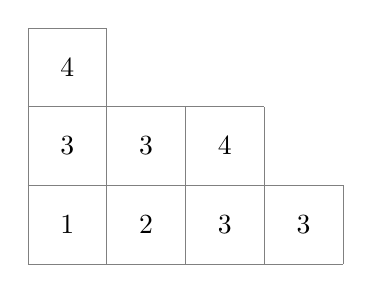
\begin{tikzpicture}
			\draw[very thin, gray] (0,2) grid (1,3);
			\draw[very thin, gray] (0,1) grid (3,2);
			\draw[very thin, gray] (0,0) grid (4,1);
			\foreach \i\j in {0/1,1/2,2/3,3/3}{
				\node at (\i+0.5, 0.5) {\j};
			}
			\foreach \i\j in {0/3,1/3,2/4}{
				\node at (\i+0.5, 1.5) {\j};
			}
			\foreach \i\j in {0/4}{
				\node at (\i+0.5, 2.5) {\j};
			}
		\end{tikzpicture}
		\caption{Tableau a}
		\label{fig:tab2}
	\end{subfigure}
	\begin{subfigure}[b]{0.4\linewidth}
		\centering
		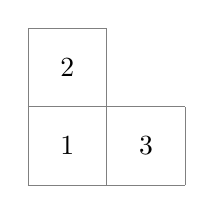
\begin{tikzpicture}
			\draw[very thin, gray] (0,2) grid (1,3);
			\draw[very thin, gray] (0,1) grid (2,2);
			\foreach \i\j in {0/1,1/3}{
				\node at (\i+0.5, 1.5) {\j};
			}
			\foreach \i\j in {0/2}{
				\node at (\i+0.5, 2.5) {\j};
			}
		\end{tikzpicture}
		\caption{Tableau b}
		\label{fig:tab3}
	\end{subfigure}
	\label{fig:tabs1}
\end{figure}
Cette section définit quelques opérations de tableau de base, qui aideront à définir la multiplication de Knuth.
\begin{definition}[taille]
	La taille $|t|$ d'un tableau $t$ est le nombre d'entrées dans le tableau.
\end{definition}
 
Par exemple, les tableaux $a$ et $b$ ont les tailles suivantes : $|a| = 8$ et  $|b| = 3$ .
Le tableau vide a une taille de 0. On note $\underline{t}$ la dernière ligne d'un tableau $t$. 
La rangée inférieure contient la plus petite entrée de chaque colonne. 
\begin{definition}[surtableau]
	Le surtableau $\overline{t}$ du tableau $t$  est le tableau qui se situe au-dessus de la rangée inférieure t.
\end{definition} 
En d'autres termes, le surtableau $\overline{t}$ est simplement t avec la rangée inférieure t retirée. Pour les tableaux d'exemple a et b , nous avons : \\
\begin{figure}[!ht]
	\centering
	\begin{subfigure}[b]{0.4\linewidth}
		\centering
		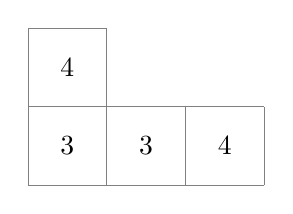
\begin{tikzpicture}
			\draw[very thin, gray] (0,2) grid (1,3);
			\draw[very thin, gray] (0,1) grid (3,2);
			\foreach \i\j in {0/3,1/3,2/4}{
				\node at (\i+0.5, 1.5) {\j};
			}
			\foreach \i\j in {0/4}{
				\node at (\i+0.5, 2.5) {\j};
			}
		\end{tikzpicture}
		\caption{Tableau $\overline{a}$}
		\label{fig:tab4}
	\end{subfigure}
	\begin{subfigure}[b]{0.4\linewidth}
		\centering
		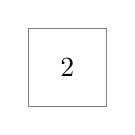
\begin{tikzpicture}
			\draw[very thin, gray] (0,2) grid (1,3);
			\foreach \i\j in {0/2}{
				\node at (\i+0.5, 2.5) {\j};
			}
		\end{tikzpicture}
		\caption{Tableau $\overline{b}$}
		\label{fig:tab5}
	\end{subfigure}
	\label{fig:tabs2}
\end{figure}
\begin{figure}[!ht]
	\centering
	\begin{subfigure}[b]{0.4\linewidth}
		\centering
		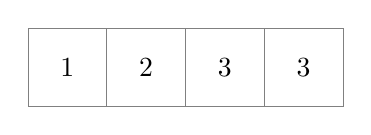
\begin{tikzpicture}
			\draw[very thin, gray] (0,2) grid (4,1);
			\foreach \i\j in {0/1,1/2,2/3,3/3}{
				\node at (\i+0.5, 1.5) {\j};
			}
		\end{tikzpicture}
		\caption{Tableau $\underline{a}$}
		\label{fig:tab6}
	\end{subfigure}
	\begin{subfigure}[b]{0.4\linewidth}
		\centering
		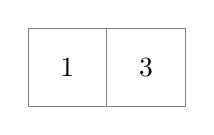
\begin{tikzpicture}
			\draw[very thin, gray] (0,2) grid (2,3);
			\foreach \i\j in {0/1,1/3}{
				\node at (\i+0.5, 2.5) {\j};
			}
		\end{tikzpicture}
		\caption{Tableau $\underline{b}$}
		\label{fig:tab7}
	\end{subfigure}
	\label{fig:tabs3}
\end{figure}
\\
$\rho$($\overline{a}$) = 4334 ,$\rho$($\overline{b}$) = 2 , $\rho$($\underline{a}$) = 1233 $\rho$($\underline{b}$) = 13 . 
Certains cas particuliers : si t n'a qu'une seule rangée, alors son surtableau est le tableau vide ; si t est vide, alors le surtableau et la rangée inférieure sont également vides. La lecture de la rangée $\rho$(t) d'un tableau t est la concaténation de toutes les rangées de t, en commençant par la rangée supérieure à gauche et en terminant par la rangée inférieure à droite. Pour les tableaux d'exemple a et b, les lectures de rangée sont les suivantes : $\rho$(a) = 43341233 $\rho$(b) = 213. Lorsque nous avons besoin de nous référer à des entrées individuelles d'un tableau, nous pouvons écrire ti pour la ième entrée de $\rho$(t), en commençant par i = 1 à gauche. 
Ainsi,$\rho(t) = t_1 t_2 \ldots t_{|t|}$ .Notez que nous écrivons parfois ti pour indiquer plusieurs tableaux différents : si le contexte n'est pas suffisant pour distinguer si ti signifie une entrée de t ou un tableau distinct, alors écrivez $\rho(t)_i$ pour la ième entrée de la lecture de rangée.
\subsubsection{La multiplication de Knuth}
\begin{algorithm}
	\caption{Insertion d'une entrée dans un tableau}
	%\SetAlgoLined
	\Entree{Tableau $t$, Entrée à insérer $u$}
	\Sortie{Tableau résultant $v$}
	\BlankLine
	Initialiser $v=t$; \\
	\Pour{$k=1$ à $|u|$}{
	Insérer l'entrée $x = u_k$ dans le tableau $v$, en utilisant les actions suivantes; \\
	\uSi{Ajouter $x$ à la rangée du bas de $v$ donne une rangée triée}{
	Remplacer la rangée du bas de $v$ par $vx$;
	}
	\Sinon{
	Soit $r$ la plus petite entrée de la rangée du bas de $v$ qui est plus grande que $x$; \\
	Remplacer la copie la plus à gauche de $r$ par $x$, en modifiant $v$; \\
	Insérer $r$ dans le surtableau $v$ (ainsi, l'entrée $x$ "pousse" l'entrée $r$ vers le haut dans les rangées supérieures);
	}
	}
	Renvoyer le tableau résultant $v$;
	\end{algorithm}

Notez que cet algorithme utilise la notion de "rangée" pour représenter une série d'éléments triés dans le tableau $v$. La première rangée de $v$ contient les éléments les plus petits, tandis que la dernière rangée contient les éléments les plus grands. Lorsqu'un nouvel élément $x$ est inséré dans $v$, l'algorithme recherche la rangée appropriée pour insérer $x$, en utilisant la méthode décrite dans les étapes c) i) et c) ii) de l'algorithme.
\subsubsection{Exemple}
\begin{figure}[!ht]
	\centering
	\begin{subfigure}[b]{0.4\linewidth}
		\centering
		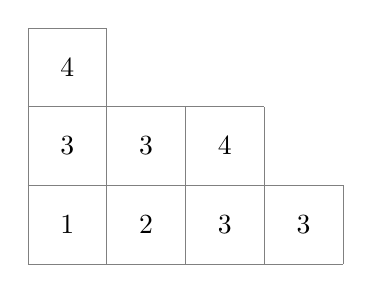
\begin{tikzpicture}
			\draw[very thin, gray] (0,2) grid (1,3);
			\draw[very thin, gray] (0,1) grid (3,2);
			\draw[very thin, gray] (0,0) grid (4,1);
			\foreach \i\j in {0/1,1/2,2/3,3/3}{
				\node at (\i+0.5, 0.5) {\j};
			}
			\foreach \i\j in {0/3,1/3,2/4}{
				\node at (\i+0.5, 1.5) {\j};
			}
			\foreach \i\j in {0/4}{
				\node at (\i+0.5, 2.5) {\j};
			}
		\end{tikzpicture}
		\caption{Tableau a}
		\label{fig:tab8}
	\end{subfigure}
	\begin{subfigure}[b]{0.4\linewidth}
		\centering
		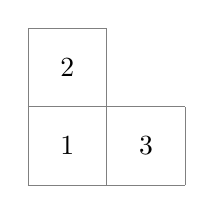
\begin{tikzpicture}
			\draw[very thin, gray] (0,2) grid (1,3);
			\draw[very thin, gray] (0,1) grid (2,2);
			\foreach \i\j in {0/1,1/3}{
				\node at (\i+0.5, 1.5) {\j};
			}
			\foreach \i\j in {0/2}{
				\node at (\i+0.5, 2.5) {\j};
			}
		\end{tikzpicture}
		\caption{Tableau b}
		\label{fig:tab9}
	\end{subfigure}
	\label{fig:tabs4}
\end{figure}
A titre d'exemple, pour multiplier les tableaux $t = a$ et $u = b$, nous prenons $v = a$ comme initialisation. 
Puisque $\rho(b) = 213$, nous devons d'abord insérer $x = b_1 = 2$ dans $v$. 
La rangée inférieure de $v$ est maintenant $1233$. 
La concaténation $vx = 12332$ n'est pas triée de façon croissante car les deux dernières entrées ont $3 > 2$. 
Nous devons donc appliquer la deuxième option d'insertion, qui fait avancer une entrée de la rangée inférieure. 
La plus petite entrée $r$ de $v$ qui est supérieure à $x = 2$ est $r = 3$. Nous remplaçons donc la rangée inférieure $1233$ par $1223$. 
Le symbole remplacé $r = 3$ est poussé vers le haut dans l'overtableau $v$. 
Pour effectuer le déplacement, nous examinons d'abord l'overtableau $w = \overline{v}$, qui est :
\begin{figure}[!ht]
	\centering
	\begin{subfigure}[b]{0.4\linewidth}
		\centering
		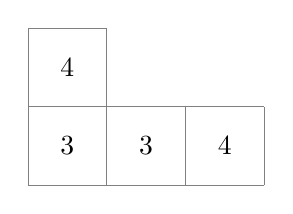
\begin{tikzpicture}
			\draw[very thin, gray] (0,2) grid (1,3);
			\draw[very thin, gray] (0,1) grid (3,2);
			\foreach \i\j in {0/3,1/3,2/4}{
				\node at (\i+0.5, 1.5) {\j};
			}
			\foreach \i\j in {0/4}{
				\node at (\i+0.5, 2.5) {\j};
			}
		\end{tikzpicture}
		\caption{Tableau w = $\overline{v}$}
		\label{fig:tab10}
	\end{subfigure}
	\label{fig:tabs5}
\end{figure}
Puisque nous essayons maintenant d'insérer 3 dans $v$, écrivons $x = 3$. 
Nous voyons que $x = 3$ ne peut pas être ajouté à la dernière ligne $w = 334$ de $v$, car $3343$ n'est pas trié. 
Une autre entrée doit être déplacée vers le haut. 
Dans ce cas, la plus petite entrée plus grande que $x = 3$ est $r = 4$, nous devons donc déplacer $4$ vers le haut. 
L'entrée déplacée, $4$, peut être ajoutée à la ligne supérieure, donnant une nouvelle ligne supérieure, $44$. 
Ainsi, après l'insertion de $2$ dans $v$, nous obtenons une nouvelle valeur pour le tableau $v$:
\begin{figure}[!ht]
	\centering
	\begin{subfigure}[b]{0.4\linewidth}
		\centering
		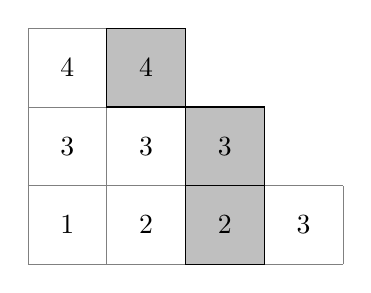
\begin{tikzpicture}
			\draw[very thin, gray] (0,2) grid (2,3);
			\draw[very thin, gray] (0,1) grid (3,2);
			\draw[very thin, gray] (0,0) grid (4,1);
			\filldraw[fill=gray!50] (2,0) rectangle (3,1);
			\filldraw[fill=gray!50] (2,1) rectangle (3,2);
			\filldraw[fill=gray!50] (1,2) rectangle (2,3);			
			\foreach \i\j in {0/1,1/2,2/2,3/3}{
				\node at (\i+0.5, 0.5) {\j};
			}
			\foreach \i\j in {0/3,1/3,2/3}{
				\node at (\i+0.5, 1.5) {\j};
			}
			\foreach \i\j in {0/4,1/4}{
				\node at (\i+0.5, 2.5) {\j};
			}
		\end{tikzpicture}
		\caption{Tableau v}
		\label{fig:tab11}
	\end{subfigure}
	\label{fig:tabs6}
\end{figure}
Les entrées modifiées sont coloré. La prochaine entrée de $b$ à insérer est $b_2 = 1$, qui doit être insérée dans ce nouveau $v$. 
En se basant sur notre expérience de l'insertion précédente, on peut voir ce qui se passe un peu plus rapidement : $1$ pousse $2$ de la première rangée (en partant du bas), ce qui pousse $3$ de la deuxième rangée, qui pousse $4$ de la troisième rangée. Cette fois, la dernière entrée poussée $4$ est ajoutée à la rangée vide ci-dessus, créant une nouvelle rangée non vide. Le nouveau $v$ est :
 \begin{figure}[!ht]
	\centering
	\begin{subfigure}[b]{0.4\linewidth}
		\centering
		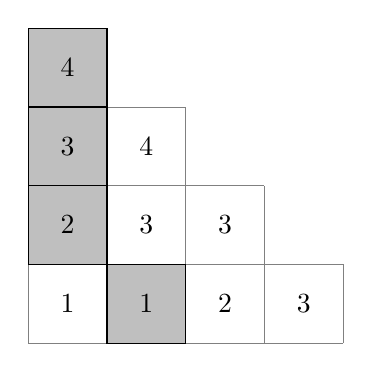
\begin{tikzpicture}
			\draw[very thin, gray] (0,3) grid (1,4);
			\draw[very thin, gray] (0,2) grid (2,3);
			\draw[very thin, gray] (0,1) grid (3,2);
			\draw[very thin, gray] (0,0) grid (4,1);
			\filldraw[fill=gray!50] (0,3) rectangle (1,4);
			\filldraw[fill=gray!50] (0,2) rectangle (1,3);
			\filldraw[fill=gray!50] (0,1) rectangle (1,2);
			\filldraw[fill=gray!50] (1,0) rectangle (2,1);
			\foreach \i\j in {0/1,1/1,2/2,3/3}{
				\node at (\i+0.5, 0.5) {\j};
			}
			\foreach \i\j in {0/2,1/3,2/3}{
				\node at (\i+0.5, 1.5) {\j};
			}
			\foreach \i\j in {0/3,1/4}{
				\node at (\i+0.5, 2.5) {\j};
			}
			\foreach \i\j in {0/4}{
				\node at (\i+0.5, 3.5) {\j};
			}
		\end{tikzpicture}
		\caption{Tableau v}
		\label{fig:tab12}
	\end{subfigure}
	\label{fig:tabs7}
\end{figure}
Les entrées modifiées sont coloré. La prochaine entrée de $b$ à insérer est $b_2 = 1$, qui doit être insérée dans ce nouveau $v$. 
En se basant sur notre expérience de l'insertion précédente, on peut voir ce qui se passe un peu plus rapidement : $1$ pousse $2$ de la première rangée (en partant du bas), ce qui pousse $3$ de la deuxième rangée, qui pousse $4$ de la troisième rangée. 
Cette fois, la dernière entrée poussée $4$ est ajoutée à la rangée vide ci-dessus, créant une nouvelle rangée non vide. Le nouveau $v$ est : \\
Les nouvelles entrées modifiées de la nouvelle $v$ ont (encore une fois) été coloré. 
Remarquez que l'entrée modifiée dans la rangée du bas est l'entrée insérée $b_2$, tandis que les entrées modifiées dans l'overtableau étaient les entrées poussées.
La dernière entrée de $b$ à insérer est $b_3 = 3$. 
Cette entrée est ajoutée à la rangée du bas (car l'ajouter donne une rangée triée), ce qui donne la nouvelle $v$, ainsi que la multiplication finale de $a$ et $b$ : 
\begin{figure}[!ht]
	\centering
	\begin{subfigure}[b]{0.4\linewidth}
		\centering
		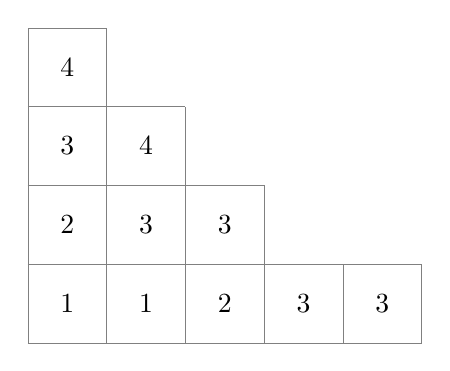
\begin{tikzpicture}
			\draw[very thin, gray] (0,2) grid (1,4);
			\draw[very thin, gray] (0,2) grid (2,3);
			\draw[very thin, gray] (0,1) grid (3,2);
			\draw[very thin, gray] (0,0) grid (5,1);
			\foreach \i\j in {0/1,1/1,2/2,3/3,4/3}{
				\node at (\i+0.5, 0.5) {\j};
			}
			\foreach \i\j in {0/2,1/3,2/3}{
				\node at (\i+0.5, 1.5) {\j};
			}
			\foreach \i\j in {0/3,1/4}{
				\node at (\i+0.5, 2.5) {\j};
			}
			\foreach \i\j in {0/4}{
				\node at (\i+0.5, 3.5) {\j};
			}
		\end{tikzpicture}
		\caption{Tableau ab = v}
		\label{fig:tab13}
	\end{subfigure}
	\label{fig:tabs8}
\end{figure}
avec la seule entrée modifiée coloré.

\subsubsection{Implémentation}
La partie difficile dans l'implémentation de la multiplication est de coder la fonction d'insertion \texttt{insert}. Dans le cas où le tableau n'est pas vide, on parcourt la liste des lignes. Pour contenir l'élèment à insérer, on utilise une variable \texttt{symb} de type \texttt{Option<Symbol>}. Le type \texttt{Option} définit dans la bibliothèque standard de Rust contient soit \texttt{None} (rien), soit une valeur.  Si \texttt{symb} est plus grand que le dernier élément de la ligne, il suffit de l'ajouter à la fin et l'insertion est terminée. Pour signifier que l'insertion est bien terminée, on met \texttt{symb} à \texttt{None}. Si \texttt{symb} n'est pas  plus grand que le dernier élément de la liste, on cherche la première valeur supérieure à \texttt{symb} dans la ligne, on met \texttt{symb} à sa place, on change la valeur de \texttt{symb} et on passe à la ligne suivante. À la fin, il se peut que l'on doive rajouter une ligne au tableau. Pour savoir si c'est le cas, on vérifie la valeur de \texttt{symb} : si elle n'est pas  à \texttt{None} c'est qu'il faut ajouter une ligne.

La multiplication est ensuite très simple puisqu'il suffit d'insérer un à un les éléments du tableau de droite dans le tableau de gauche. Pour effectuer la recherche du premier symbole supérieur à \texttt{symb} dans l'insertion, nous avons codé une fonction de recherche dichotomique qui renvoie l'indice dans la ligne de l'élément recherché.

\subsubsection{Tests}
Nous avons testé fait des tests à partir d'exemples calculés à la main. On vérifie aussi certainnes propriétés, par exemple le fait qu'on ait bien $t=P(\rho(t))$ ou que le tableau vide soit bien l'élément neutre.

\subsection{La division par érosion}
Cette section explique la division par érosion, qui est un algorithme pour diviser des tableaux semi-standard, présenté dans ce rapport.

L'érosion de $b$ à partir de $d = ab$ consiste à essayer de supprimer les entrées de $b$ de $d$, une par une, dans l'ordre inverse de leur insertion. Chaque suppression fait descendre les entrées dans le tableau, en commençant par un pic dans le tableau. L'érosion essaie chaque pic de $d$ pour voir s'il supprime la dernière entrée $x$ de $b$ qui doit être supprimée. En cas de correspondance, elle utilise récursivement l'érosion pour supprimer plus d'entrées de $b$ de $d$.

Chaque fois qu'une correspondance échoue, l'érosion revient en arrière sur la suppression tentée et essaie de supprimer et d'éroder récursivement à partir d'un nouveau pic de $d$.

Notez la terminologie métaphorique suivante.
Le terme "plactic" est lié à la tectonique des plaques. 
La multiplication des tableaux ressemble un peu à la collision de deux montagnes qui fusionnent en une montagne plus grande. En revanche, l'érosion correspond au processus inverse, la plus grande montagne s'érodant pour devenir une montagne plus petite. Plus spécifiquement, l'algorithme d'érosion essaie de supprimer des petites pièces aléatoires de la plus grande montagne, en poussant vers le bas à partir de différents points de la surface supérieure de la montagne. 
La suppression des lignes peut être considérée comme un courant, érodant la montagne.

\subsubsection{Pics d'un tableau}
Un pic $p$ d'un tableau est une entrée $p$ sans entrée au-dessus et sans entrée à droite. 
Équivalament, un pic est une entrée qui est à la fois le haut d'une colonne et la fin d'une ligne.
En d'autres termes, un pic est un coin supérieur droit d'un tableau.

Par exemple, le tableau $d = ab$ a quatre pics, qui sont indiqués en gras ci-dessous :
\begin{figure}[!ht]
	\centering
	\begin{subfigure}[b]{0.4\linewidth}
		\centering
		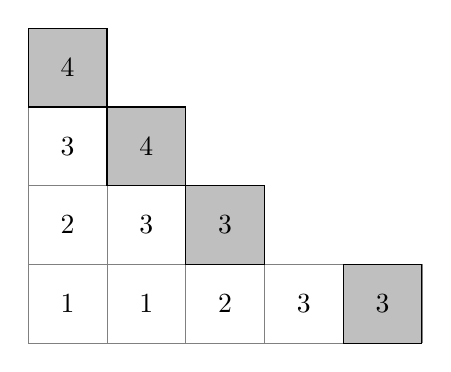
\begin{tikzpicture}
			\draw[very thin, gray] (0,2) grid (1,4);
			\draw[very thin, gray] (0,2) grid (2,3);
			\draw[very thin, gray] (0,1) grid (3,2);
			\draw[very thin, gray] (0,0) grid (5,1);
			\filldraw[fill=gray!50] (4,0) rectangle (5,1);
			\filldraw[fill=gray!50] (2,1) rectangle (3,2);
			\filldraw[fill=gray!50] (1,2) rectangle (2,3);
			\filldraw[fill=gray!50] (0,3) rectangle (1,4);
			\foreach \i\j in {0/1,1/1,2/2,3/3,4/3}{
				\node at (\i+0.5, 0.5) {\j};
			}
			\foreach \i\j in {0/2,1/3,2/3}{
				\node at (\i+0.5, 1.5) {\j};
			}
			\foreach \i\j in {0/3,1/4}{
				\node at (\i+0.5, 2.5) {\j};
			}
			\foreach \i\j in {0/4}{
				\node at (\i+0.5, 3.5) {\j};
			}
		\end{tikzpicture}
		\caption{Tableau d}
		\label{fig:tab14}
	\end{subfigure}
	\label{fig:tabs9}
\end{figure}
Lorsqu'on insère une nouvelle entrée $x$ dans un tableau $v$ pour obtenir un tableau plus grand $w$, la dernière entrée de $w$ à être modifiée sera un pic de $w$. Ce nouveau pic est la seule entrée de $w$ dans une nouvelle position qui n'était pas occupée dans $v$. En d'autres termes, l'insertion se termine toujours à un (nouveau) pic. Cette perspective suggère que les pics devraient être le point de départ pour le processus inverse à l'insertion.

Il convient de noter que différents pics peuvent avoir la même valeur, de sorte que le pic inclut la position de l'entrée, pas seulement sa valeur.

\subsubsection{Suppression}
La suppression, définie ci-dessous, commence à un pic donné $p$ d'un tableau $t$ donné, 
et se termine en produisant un tableau plus petit $s$ (une modification de $t$) et en supprimant une entrée $x$ de la rangée inférieure de $t$. 
En d'autres termes, l'entrée $t$ et le pic $p$ sont les entrées, et le tableau $s$ et l'entrée supprimée $x$ sont les sorties.\\
\begin{algorithm}
	\Entree{tableau $t$, pic $p$}
	\Sortie{tableau $s$ et entrée supprimée $x$}
	Initialiser $s$ avec les éléments de $t$; \\
	Initialiser $x$ avec la valeur de l'entrée $p$; \\
	Soit $r$ un entier positif tel que $p$ soit dans la rangée $r$ de $s$ (la rangée du bas est la rangée 1, et ensuite on compte vers le haut); \\
	Supprimer $p$ de (la fin de) la rangée $r$ de $s$ (donc maintenant $|s| = |t| - 1$); \\
	\Tq{$r > 1$}{
	Réduire $r$ de 1; \\
	Dans la rangée $r$ de $s$, laisser $y$ être l'entrée la plus grande avec $y < x$; \\
	Dans la rangée $r$ de $s$, remplacer la copie la plus à droite de $y$ par $x$; \\
	Mettre à jour $x$ avec la valeur $y$; 
	}
	\Retour{$s$ et la valeur finale de l'entrée $x$}
	\caption{Algorithme de suppression}
\end{algorithm}
Notez que la suppression est l'opposé de l'insertion, dans le sens où l'insertion de l'entrée $x$ dans $s$ donne $t$.\\
\subsubsection{Exemple}
Chacun des quatre pics donne lieu à sa propre suppression, qui est illustrée ci-dessous :
\begin{figure}[!ht]
	\centering
	\begin{subfigure}[b]{0.4\linewidth}
		\centering
		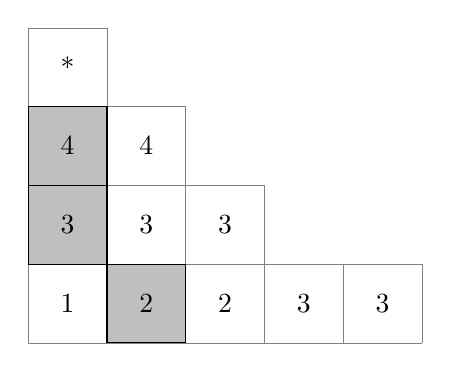
\begin{tikzpicture}
			\draw[very thin, gray] (0,3) grid (1,4);
			\draw[very thin, gray] (0,2) grid (2,3);
			\draw[very thin, gray] (0,1) grid (3,2);
			\draw[very thin, gray] (0,0) grid (5,1);
			\filldraw[fill=gray!50] (1,0) rectangle (2,1);
			\filldraw[fill=gray!50] (0,1) rectangle (1,2);
			\filldraw[fill=gray!50] (0,2) rectangle (1,3);
			\foreach \i\j in {0/1,1/2,2/2,3/3,4/3}{
				\node at (\i+0.5, 0.5) {\j};
			}
			\foreach \i\j in {0/3,1/3,2/3}{
				\node at (\i+0.5, 1.5) {\j};
			}
			\foreach \i\j in {0/4,1/4}{
				\node at (\i+0.5, 2.5) {\j};
			}
			\foreach \i\j in {0/*}{
				\node at (\i+0.5, 3.5) {\j};
			}
		\end{tikzpicture}
		\caption{la suppression de 1}
		\label{fig:tab15}
	\end{subfigure}
	\begin{subfigure}[b]{0.4\linewidth}
		\centering
		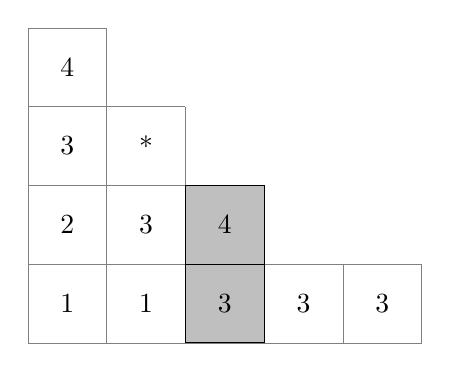
\begin{tikzpicture}
			\draw[very thin, gray] (0,3) grid (1,4);
			\draw[very thin, gray] (0,2) grid (2,3);
			\draw[very thin, gray] (0,1) grid (3,2);
			\draw[very thin, gray] (0,0) grid (5,1);
			\filldraw[fill=gray!50] (2,0) rectangle (3,1);
			\filldraw[fill=gray!50] (2,1) rectangle (3,2);
			\foreach \i\j in {0/1,1/1,2/3,3/3,4/3}{
				\node at (\i+0.5, 0.5) {\j};
			}
			\foreach \i\j in {0/2,1/3,2/4}{
				\node at (\i+0.5, 1.5) {\j};
			}
			\foreach \i\j in {0/3,1/*}{
				\node at (\i+0.5, 2.5) {\j};
			}
			\foreach \i\j in {0/4}{
				\node at (\i+0.5, 3.5) {\j};
			}
		\end{tikzpicture}
		\caption{la suppression de 2}
		\label{fig:tab16}
	\end{subfigure}
	\label{fig:tab17}
	\begin{subfigure}[b]{0.4\linewidth}
		\centering
		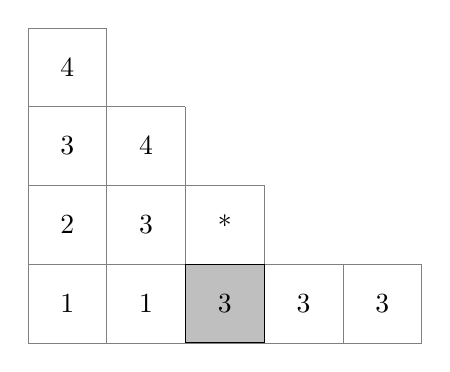
\begin{tikzpicture}
			\draw[very thin, gray] (0,3) grid (1,4);
			\draw[very thin, gray] (0,2) grid (2,3);
			\draw[very thin, gray] (0,1) grid (3,2);
			\draw[very thin, gray] (0,0) grid (5,1);
			\filldraw[fill=gray!50] (2,0) rectangle (3,1);
			\foreach \i\j in {0/1,1/1,2/3,3/3,4/3}{
				\node at (\i+0.5, 0.5) {\j};
			}
			\foreach \i\j in {0/2,1/3,2/*}{
				\node at (\i+0.5, 1.5) {\j};
			}
			\foreach \i\j in {0/3,1/4}{
				\node at (\i+0.5, 2.5) {\j};
			}
			\foreach \i\j in {0/4}{
				\node at (\i+0.5, 3.5) {\j};
			}
		\end{tikzpicture}
		\caption{la suppression de 2}
		\label{fig:tab18}
	\end{subfigure}
	\label{fig:tab19}
	\begin{subfigure}[b]{0.4\linewidth}
		\centering
		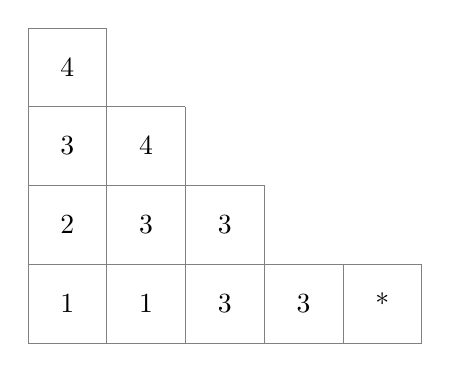
\begin{tikzpicture}
			\draw[very thin, gray] (0,3) grid (1,4);
			\draw[very thin, gray] (0,2) grid (2,3);
			\draw[very thin, gray] (0,1) grid (3,2);
			\draw[very thin, gray] (0,0) grid (5,1);
			\foreach \i\j in {0/1,1/1,2/3,3/3,4/*}{
				\node at (\i+0.5, 0.5) {\j};
			}
			\foreach \i\j in {0/2,1/3,2/3}{
				\node at (\i+0.5, 1.5) {\j};
			}
			\foreach \i\j in {0/3,1/4}{
				\node at (\i+0.5, 2.5) {\j};
			}
			\foreach \i\j in {0/4}{
				\node at (\i+0.5, 3.5) {\j};
			}
		\end{tikzpicture}
		\caption{la suppression de 3}
		\label{fig:tab20}
	\end{subfigure}
	\label{fig:tabs12}
\end{figure}
\pagebreak

Le nouveau tableau plus petit s'est présenté au-dessus de la ligne, et l'entrée supprimée x est présentée en dessous de la ligne. 
Les entrées de s qui ont subi un remplacement sont indiquées. 
La position précédente du pic de $t$ est indiquée par *. 
Le pic * n'est pas une entrée de s.
Remarquez que le fait de faire glisser les caractères coloré d'une ligne vers le haut montre le processus de réinsertion de l'entrée supprimée. 
En faisant référence à la métaphore de l'érosion, les caractères coloré indiquent le chemin d'un cours d'eau dans l'érosion de la montagne

\subsubsection{Division par érosion}
La division par érosion consiste à diviser le tableau d par le tableau b en appliquant l'érosion du tableau d par le mot $\rho(b)$ (la lecture des rangées de b). 
Plus généralement, on peut utiliser l'érosion de d par n'importe quel mot w représentant b, ce qui signifie que P(w) = b.

\subsubsection{Exemple}
Nous allons maintenant diviser le tableau $d = ab$  par le tableau $b$ . Comme $\rho(b) = 213$, nous devons supprimer $m = 3$ entrées. La première entrée à supprimer est $b_3 = 3$.

Les quatre pics de $d$ ont déjà été listés , et les résultats des suppressions de ces quatre pics ont également été énumérés. Seul l'un des quatre pics conduit à la suppression de $b_3 = 3$, qui se trouve être le pic le plus bas (le plus à droite).

La suppression de 3 nous donne un tableau $s$ plus petit qui a également quatre pics. Les suppressions des quatre pics de $s$ sont les suivantes :

\begin{figure}[!ht]
	\centering
	\begin{subfigure}[b]{0.4\linewidth}
		\centering
		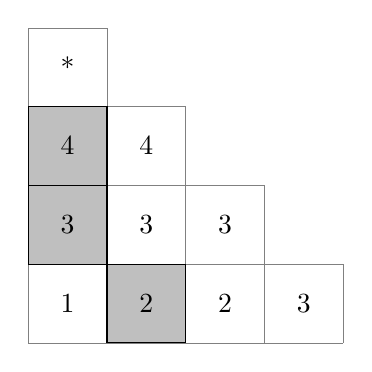
\begin{tikzpicture}
			\draw[very thin, gray] (0,3) grid (1,4);
			\draw[very thin, gray] (0,2) grid (2,3);
			\draw[very thin, gray] (0,1) grid (3,2);
			\draw[very thin, gray] (0,0) grid (4,1);
			\filldraw[fill=gray!50] (1,0) rectangle (2,1);
			\filldraw[fill=gray!50] (0,1) rectangle (1,2);
			\filldraw[fill=gray!50] (0,2) rectangle (1,3);
			\foreach \i\j in {0/1,1/2,2/2,3/3}{
				\node at (\i+0.5, 0.5) {\j};
			}
			\foreach \i\j in {0/3,1/3,2/3}{
				\node at (\i+0.5, 1.5) {\j};
			}
			\foreach \i\j in {0/4,1/4}{
				\node at (\i+0.5, 2.5) {\j};
			}
			\foreach \i\j in {0/*}{
				\node at (\i+0.5, 3.5) {\j};
			}
		\end{tikzpicture}
		\caption{la suppression de 1}
		\label{fig:tab21}
	\end{subfigure}
	\begin{subfigure}[b]{0.4\linewidth}
		\centering
		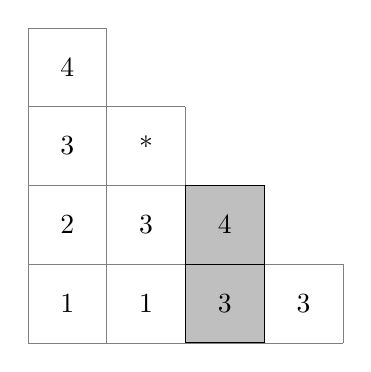
\begin{tikzpicture}
			\draw[very thin, gray] (0,3) grid (1,4);
			\draw[very thin, gray] (0,2) grid (2,3);
			\draw[very thin, gray] (0,1) grid (3,2);
			\draw[very thin, gray] (0,0) grid (4,1);
			\filldraw[fill=gray!50] (2,0) rectangle (3,1);
			\filldraw[fill=gray!50] (2,1) rectangle (3,2);
			\foreach \i\j in {0/1,1/1,2/3,3/3}{
				\node at (\i+0.5, 0.5) {\j};
			}
			\foreach \i\j in {0/2,1/3,2/4}{
				\node at (\i+0.5, 1.5) {\j};
			}
			\foreach \i\j in {0/3,1/*}{
				\node at (\i+0.5, 2.5) {\j};
			}
			\foreach \i\j in {0/4}{
				\node at (\i+0.5, 3.5) {\j};
			}
		\end{tikzpicture}
		\caption{la suppression de 2}
		\label{fig:tab22}
	\end{subfigure}
	\label{fig:tab23}
	\begin{subfigure}[b]{0.4\linewidth}
		\centering
		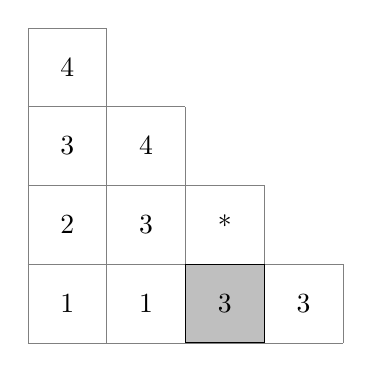
\begin{tikzpicture}
			\draw[very thin, gray] (0,3) grid (1,4);
			\draw[very thin, gray] (0,2) grid (2,3);
			\draw[very thin, gray] (0,1) grid (3,2);
			\draw[very thin, gray] (0,0) grid (4,1);
			\filldraw[fill=gray!50] (2,0) rectangle (3,1);
			\foreach \i\j in {0/1,1/1,2/3,3/3}{
				\node at (\i+0.5, 0.5) {\j};
			}
			\foreach \i\j in {0/2,1/3,2/*}{
				\node at (\i+0.5, 1.5) {\j};
			}
			\foreach \i\j in {0/3,1/4}{
				\node at (\i+0.5, 2.5) {\j};
			}
			\foreach \i\j in {0/4}{
				\node at (\i+0.5, 3.5) {\j};
			}
		\end{tikzpicture}
		\caption{la suppression de 2}
		\label{fig:tab24}
	\end{subfigure}
	\label{fig:tab25}
	\begin{subfigure}[b]{0.4\linewidth}
		\centering
		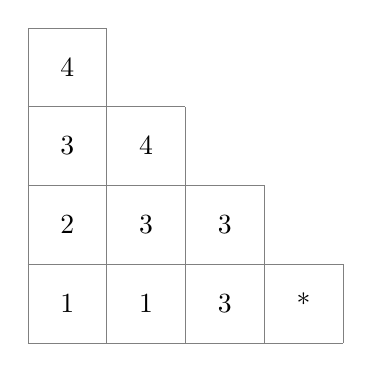
\begin{tikzpicture}
			\draw[very thin, gray] (0,3) grid (1,4);
			\draw[very thin, gray] (0,2) grid (2,3);
			\draw[very thin, gray] (0,1) grid (3,2);
			\draw[very thin, gray] (0,0) grid (4,1);
			\foreach \i\j in {0/1,1/1,2/3,3/*}{
				\node at (\i+0.5, 0.5) {\j};
			}
			\foreach \i\j in {0/2,1/3,2/3}{
				\node at (\i+0.5, 1.5) {\j};
			}
			\foreach \i\j in {0/3,1/4}{
				\node at (\i+0.5, 2.5) {\j};
			}
			\foreach \i\j in {0/4}{
				\node at (\i+0.5, 3.5) {\j};
			}
		\end{tikzpicture}
		\caption{la suppression de 3}
		\label{fig:tab26}
	\end{subfigure}
	\label{fig:tabs13}
\end{figure}
La prochaine entrée à supprimer est b2 = 1, mais le seul pic de s qui conduit à la suppression de 1 est le pic le plus élevé (le plus à gauche). Donc, maintenant nous continuons le processus d'érosion à partir du tableau le plus à gauche des quatre choix ci-dessus.

Le nouveau tableau s plus petit a 3 pics, qui sont supprimés comme suit :
\begin{figure}[!ht]
	\centering
	\begin{subfigure}[b]{0.4\linewidth}
		\centering
		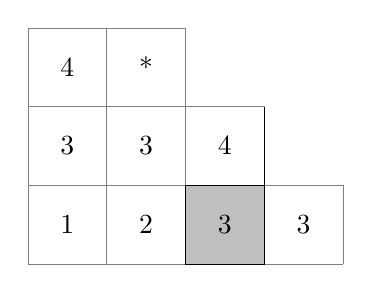
\begin{tikzpicture}
			\draw[very thin, gray] (0,2) grid (2,3);
			\draw[very thin, gray] (0,1) grid (3,2);
			\draw[very thin, gray] (0,0) grid (4,1);
			\filldraw[fill=gray!50] (2,0) rectangle (3,1);
			\filldraw[fill=gray!50] (3,1) rectangle (3,2);
			\foreach \i\j in {0/1,1/2,2/3,3/3}{
				\node at (\i+0.5, 0.5) {\j};
			}
			\foreach \i\j in {0/3,1/3,2/4}{
				\node at (\i+0.5, 1.5) {\j};
			}
			\foreach \i\j in {0/4,1/*}{
				\node at (\i+0.5, 2.5) {\j};
			}
		\end{tikzpicture}
		\caption{la suppression de 2}
		\label{fig:tab27}
	\end{subfigure}
	\begin{subfigure}[b]{0.4\linewidth}
		\centering
		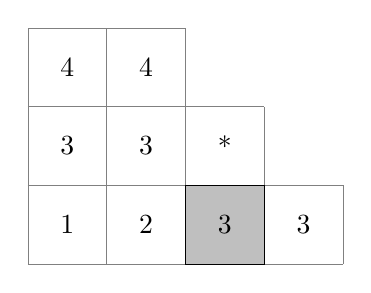
\begin{tikzpicture}
			\draw[very thin, gray] (0,2) grid (2,3);
			\draw[very thin, gray] (0,1) grid (3,2);
			\draw[very thin, gray] (0,0) grid (4,1);
			\filldraw[fill=gray!50] (2,0) rectangle (3,1);
			\foreach \i\j in {0/1,1/2,2/3,3/3}{
				\node at (\i+0.5, 0.5) {\j};
			}
			\foreach \i\j in {0/3,1/3,2/*}{
				\node at (\i+0.5, 1.5) {\j};
			}
			\foreach \i\j in {0/4,1/4}{
				\node at (\i+0.5, 2.5) {\j};
			}

		\end{tikzpicture}
		\caption{la suppression de 2}
		\label{fig:tab28}
	\end{subfigure}
	\label{fig:tabs15}
	\begin{subfigure}[b]{0.4\linewidth}
		\centering
		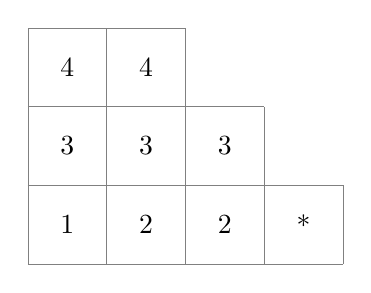
\begin{tikzpicture}
			\draw[very thin, gray] (0,2) grid (2,3);
			\draw[very thin, gray] (0,1) grid (3,2);
			\draw[very thin, gray] (0,0) grid (4,1);
			\foreach \i\j in {0/1,1/2,2/2,3/*}{
				\node at (\i+0.5, 0.5) {\j};
			}
			\foreach \i\j in {0/3,1/3,2/3}{
				\node at (\i+0.5, 1.5) {\j};
			}
			\foreach \i\j in {0/4,1/4}{
				\node at (\i+0.5, 2.5) {\j};
			}
		\end{tikzpicture}
		\caption{la suppression de 3}
		\label{fig:tab29}
	\end{subfigure}
	\label{fig:tabs16}
\end{figure}
\pagebreak

La prochaine entrée de $b$ à supprimer est $b1 = 2$. 
Nous constatons que la suppression de deux pics entraîne la suppression de 2. 
L'érosion donnera l'un de ces résultats en fonction de l'ordre des pics dans la boucle d'itération sur les pics. 
La suppression à partir du pic le plus élevé de $s$ redonne le tableau original $a$. 
Mais supposons que nous utilisons un ordre différent des pics, de sorte que nous finissons par supprimer le deuxième pic le plus élevé de $s$.
Ensuite, la division par érosion donnerait une réponse finale de:
\begin{figure}[!ht]
	\centering
	\begin{subfigure}[b]{0.4\linewidth}
		\centering
		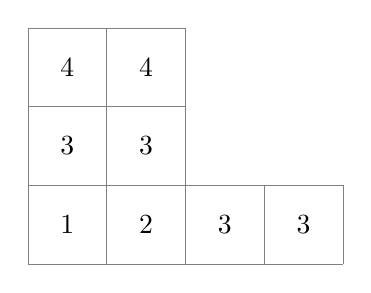
\begin{tikzpicture}
			\draw[very thin, gray] (0,2) grid (2,3);
			\draw[very thin, gray] (0,1) grid (2,2);
			\draw[very thin, gray] (0,0) grid (4,1);
			\foreach \i\j in {0/1,1/2,2/3,3/3}{
				\node at (\i+0.5, 0.5) {\j};
			}
			\foreach \i\j in {0/3,1/3}{
				\node at (\i+0.5, 1.5) {\j};
			}
			\foreach \i\j in {0/4,1/4}{
				\node at (\i+0.5, 2.5) {\j};
			}
		\end{tikzpicture}
		\caption{Tableau d/b}
		\label{fig:tab30}
	\end{subfigure}
	\label{fig:tabs17}
\end{figure} \\

\subsubsection{Érosion d'un tableau par mot}
L'érosion prend en entrée un tableau $v$ et un mot $b = b_1 . . . b_m$. Soit elle échoue, 
soit elle renvoie en sortie un tableau plus petit $t$.

L'érosion est une procédure récursive. L'érosion de $v$ par $b$ nécessitera l'érosion de tableaux plus petits par des mots plus courts. 
Le nombre de sous-érosions nécessaires peut être important, 
et le nombre exact semble difficile à prédire. Il est plus facile de décrire l'érosion comme une procédure récursive plutôt que comme une procédure itérative.

Pour éroder le tableau $v$ par le mot $b_1 . . . b_m$, faites ce qui suit:


\begin{algorithm}
 \caption{Erosion d'un tableau $v$ par le mot $b = b_1 \ldots b_m$}
 \Donnees 
 {tableau $v$ de longueur $n$, mot $b$ de longueur $m$ \\
 tableau $t$ de longueur $n'$ (si l'érosion réussit)}
 \Si{$m = 0$}
 {
 $t \gets v$ \\
 \Retour $t$
 }
 \Pour{$p \gets 1 \text{ to } n$}
 { 
 Appliquer la suppression à $v$ à partir de $p$, obtenant le tableau $s$ et l'entrée supprimée $x$ \\
 \Si{$x = b_m$} 
 {
 Exécuter récursivement l'érosion sur le tableau $s$ par le mot $c = b_1 \ldots b_{m-1}$, obtenant le tableau $q$ \\
 \Si{érosion de $s$ par $c$ réussit} 
 {
 $t \gets q$ \\
 \Retour $t$
 }
 }
 }
 Indiquer l'échec de l'érosion de $v$ par $b$
\end{algorithm}
 
 Dans cet algorithme, l'étape (a) correspond à l'application de la suppression à partir du sommet $p$, 
 ce qui donne le tableau $s$ et l'entrée supprimée $x$. L'étape (b) correspond au test sur $x$, 
 pour savoir si l'on continue ou pas. L'étape (c) correspond à l'appel récursif de l'érosion sur le tableau $s$ avec le mot $c$, 
 suivi du test sur le résultat. 
 Enfin, l'étape à la fin correspond à l'indication de l'échec de l'érosion si aucun tableau de sortie n'a été obtenu.

\subsubsection{Implementation sur le rust}
Le code fourni contient plusieurs fonctions qui implémentent l'algorithme de division par erosion en utilisant des tableaux semi-standards.
 Dans cette section, nous allons expliquer les différentes fonctions et leur utilité. \\
\textbf{Fonctions principales :}
\begin{enumerate}
\item La fonction \verb|delete_peaks| :
Cette fonction supprime un pic dans un tableau semi-standard en effectuant une opération d'érosion. Elle prend en entrée un tableau semi-standard \verb|tab1|, un index de ligne \verb|i| et un index de colonne \verb|j|. Elle retourne la valeur de l'élément supprimé \verb|sauv|.
\item La fonction \verb|erosion| :
Cette fonction applique une opération d'érosion pour supprimer tous les pics d'un tableau semi-standard. Elle prend en entrée deux tableaux semi-standards \verb|tab1| et \verb|tab2|. Elle ne retourne pas de valeur.
\end{enumerate}

\textbf{Utilisation :}

Ces fonctions sont utilisées pour effectuer une opération d'érosion sur un tableau semi-standard. L'érosion est une opération qui supprime tous les pics d'un tableau semi-standard en appliquant la méthode d'érosion de Schützenberger.

La fonction \verb|delete_peaks| est utilisée pour supprimer un pic à partir d'un index de ligne et d'un index de colonne spécifiés. Cette fonction est appelée par la fonction \verb|erosion| pour supprimer les pics dans chaque ligne du tableau semi-standard.

La fonction \verb|erosion| est utilisée pour appliquer l'opération d'érosion à deux tableaux semi-standards. Elle utilise la fonction \verb|delete_peaks| pour supprimer les pics dans chaque ligne du tableau \verb|tab1|. Ensuite, elle transpose le tableau \verb|tab1| et l'assigne au tableau \verb|tab2|. Elle répète l'opération de suppression de pics sur chaque ligne de \verb|tab2|, puis transpose à nouveau \verb|tab2| et l'assigne à \verb|tab1|. Cette opération est répétée jusqu'à ce qu'il n'y ait plus de pics dans le tableau semi-standard.

La fonction \verb|erosion| ne retourne pas de valeur, car elle modifie les tableaux \verb|tab1| et \verb|tab2| directement.

\subsubsection{La division par essai multiplication}
La division par essai multiplication consiste à calculer $d/b$ de la manière suivante : utiliser une méthode rapide pour générer un tableau à partir d'une longue liste de tableaux $[a_1, ..., a_L]$. Commencer une boucle de $i = 1$ à $i = L$ (qui peut se terminer tôt). Calculer $d_i = a_i \cdot b$ à chaque itération. Si $d_i = d$, alors s'arrêter et donner $a_i$ en sortie comme valeur pour $d/b$. Si aucune itération n'a $d_i = d$, alors signaler l'échec de la division.

Plus précisément, un algorithme de division utilise l'essai multiplication si la grande majorité de ses calculs en temps d'exécution est consacrée aux multiplications de tableau $d_i = a_i \cdot b$. (Ainsi, un algorithme de division qui consacre plus de temps à la génération des $a_i$ qu'à leur test n'est pas considéré comme une multiplication d'essai. En particulier, la division par érosion, qui passe beaucoup de temps à générer une liste de tableau $[a_1]$, n'est pas considérée comme une multiplication d'essai.)

L'essai multiplication est strict si la liste de recherche $[a_1, ..., a_L]$ ne dépend pas de $d$. Plus précisément, l'essai multiplication stricte peut générer $[a_1, ..., a_L]$ en fonction d'informations a priori sur la méthode utilisée pour générer $a$, telles que la variable aléatoire d'Alice qu'elle utilise pour générer $a$ - mais l'essai multiplication stricte ne peut pas dépendre de toute information spécifique à l'instance cible de la génération de $a$, ce qui inclut $d = ab$.

Pour les petites valeurs de $a$, ou pour $a$ généré à partir d'un petit ensemble de grands tableaux, l'essai multiplication peut être plus rapide que l'érosion.

Le reste de cette section aborde certains détails de l'essai multiplication, tels que la manière de générer la liste de recherche $[a_1, a_2, ..., a_L]$.
\subsubsection{Augmentation de la probabilté de la success}
La division par essai multiplication est garantie de réussir si l'on peut garantir que la liste de recherche contient le $a$ utilisé pour générer l'entrée $d=ab$, 
définissant ainsi l'instance du problème de division. 
Nous supposons que la liste de recherche garantit toujours la présence de $a$. Si une liste $[a_1,...,a_L]$ ne le garantit pas, 
il est généralement simple d'étendre la liste pour s'assurer qu'elle couvre tous les $a$ qui peuvent être utilisés pour générer l'instance du problème.
\subsubsection{Implementation sur le rust}
Le code fourni contient plusieurs fonctions qui implémentent un algorithme de multiplication rapide en utilisant des tableaux semi-standards. Dans cette section, 
nous allons expliquer les différentes fonctions et leur utilité.

\textbf{Fonctions principales :}
\begin{enumerate}
	\item La fonction \verb|T| :
	Cette fonction échange les valeurs des éléments \verb|w[1]| et \verb|w[(i+1)%3]|. Elle prend en entrée un entier \verb|i| et un tableau \verb|w| de taille 3. Elle retourne une valeur booléenne \verb|true|.
	\item La fonction \verb|knuth| :
	Cette fonction vérifie si la condition de Knuth est satisfaite pour \verb|i| et \verb|w|, puis appelle la fonction \verb|T| si c'est le cas. Elle prend en entrée un entier \verb|i| et un tableau \verb|w| de taille 3. Elle retourne une valeur booléenne \verb|true| si la condition de Knuth est satisfaite et que la fonction \verb|T| a été appelée, sinon elle retourne \verb|false|.

	\item La fonction \verb|robinson| :
	Cette fonction effectue une permutation de Robinson sur le tableau \verb|w| en modifiant \verb|w| directement. Elle prend en entrée un tableau \verb|w| de taille \verb|n| et un entier \verb|j|. Cette fonction est appelée dans la fonction \verb|multiplication| pour chaque élément de la nouvelle colonne.

	\item La fonction \verb|transform_to_vec_of_vecs| :
	Cette fonction transforme un vecteur de nombres en un vecteur de vecteurs où chaque vecteur interne contient une séquence croissante de nombres. Elle prend en entrée un vecteur \verb|v| de taille \verb|n|. Elle retourne un vecteur de vecteurs.

	\item La fonction \verb|multiplication| :
	Cette fonction calcule le produit de deux vecteurs et applique la permutation de Robinson pour chaque élément de la nouvelle colonne. Elle prend en entrée deux vecteurs \verb|tab1| et \verb|tab2| de tailles \verb|m| et \verb|n| respectivement. Elle retourne un vecteur de taille \verb|(m+n)|.

	\item La fonction \verb|to_semistandard_tableau| :
	Cette fonction convertit une liste de nombres en un tableau semi-standard. Elle prend en entrée un vecteur \verb|numbers| de taille \verb|n|. Elle retourne un tableau semi-standard.
\end{enumerate}

\textbf{Utilisation :}
L'algorithme est utilisé pour effectuer une division en utilisant la multiplication rapide avec des tableaux semi-standards. 
L'idée principale de l'algorithme est d'utiliser une méthode rapide pour générer une liste de tableaux semi-standards à partir d'une liste de nombres,
 puis d'appliquer la multiplication rapide pour effectuer la division. 
Si la division est réussie, l'algorithme retourne la valeur d/b, sinon il retourne un message d'erreur.
\pagebreak
\subsection{La division de Monico}
Comme nous l'avons évoqué dans la section \ref{etat_recherche}, Chris Monico, chercheur à la Texas Tech University, publia dans~\cite{monico2022division} deux algorithmes probabilistes de division dans le monoïde plaxique. Nous allons dans cette section présenter le principe de ces algorithmes et la manière dont nous les avons implémentés.

\subsubsection{Principe}
Monico commence par définir une pseudo-distance sur $\A$. Pour un mot $m \in \A$ et un entier positif $r$, on note $P_r(m) \in \A$ la $r$-ième ligne du tableau $P(m)$. Et pour $s \in \AN$, on note $|m|_s$ le nombre d'occurrences du symbole $s$ dans $m$. La distance entre $u,v \in \A$ est alors : 
\begin{definition}[distance]
	$$d(u,v) = \frac{1}{2}\sum_{r=1}^{N}\sum_{s=1}^{N}\bigl||P_r(u)|_s - |P_r(v)_s|\bigr|$$
\end{definition}

Il s'agit de la somme sur toutes les lignes et tous les symboles de la différence absolue entre le nombre d'occurrences du symbole sur la ligne dans les deux tableaux.

\begin{property} \label{prop:dist}
	La distance entre deux mots de même longueur est un entier.
\end{property}

Avant de continuer d'arriver à l'algorithme, nous nous devons de faire certains rappels mathématiques.
\begin{definition}[groupe symmétrique]
	Pour un entier positif $n$, le groupe symétrique d'ordre $n$ $S_n$ est l'ensemble des bijections de $[\![1;n]\!]$ dans $[\![1;n]\!]$.
\end{definition}
\begin{definition}[permutation]
	Une permutation $\sigma$ est un élément de $S_n$.
\end{definition}
\begin{definition}[cycle]
	Soit $n$ un entier strictement positif et $\sigma$ une permutation de $S_n$. On dit que $\sigma$ est un cycle s'il existe $p \in [\![0;n]\!]$, $i_1,...,i_p \in [\![1;n]\!]$ distincts tels que $\sigma(i_1)=i_2$, $\sigma(i_2)=i_3$, ..., $\sigma(i_{p-1})=i_p$, $\sigma(i_p)=i_1$ et $\sigma(x)=x$ si $x \notin \{i_1,...,i_p\}$. On note alors $\sigma=(i_1\ i_2\ ...\ i_p)$
\end{definition}

Posons maintenant quelques définitions et notations qui nous seront utiles pour les algorithmes de Monico. Soit $m \in \A$.
\begin{definition}[support]
	Le support de $m$ noté $\text{supp}(m)$ est l'ensemble de tous les symboles de $\AN$ apparaissant au moins une fois dans $m$.
\end{definition}
\begin{definition} \label{def:f}
	On pose alors pour tous $m \in \A$ et pour tous $s \in \AN\ {f_s(m) = |\text{supp}(m) \cap \{1,2,...,s\}|}$.
\end{definition} 
Cela nous permet de définir
\begin{definition} \label{def:D}
	$D(m) = \displaystyle\sum_{s=1}^N(f_s(m)-1)\textrm{min}(f_s(m), |m|_s)$.
\end{definition}
\begin{property} \label{prop:D}
	$D(m)$ est un majorant du  nombre de $[x] \in \P$ telles que $d(m,x)=1$
\end{property}

On rappelle que l'on essaye de résoudre le problème \ref{prob:div}, c'est-à-dire trouver $[q]$ telle que $[q][b]=[c]$. On note $n=|q|$.

L'idée de Monico est la suivante : il commence par définir un petit ensemble de permutations $\Sigma_n \subset S_n$ tel que $d(\sigma(q),q)$ soit petit et strictement positif pour tout $\sigma \in \Sigma_n$. $d(\sigma(q)b,qb)$ devrait alors généralement être petit et strictement positif. 

L'ensemble $\Sigma_n$ est défini ainsi : 
\begin{definition}[$\Sigma_n$] \label{def:Sigma_n}
	Pour $i,j \in [\![1;n]\!]$ avec $i<j$, on définit $\sigma_{ij}$ comme étant le cycle $(j\ j\!-\!1\ j\!-\!2\ ...\ i\!+\!1\ i)$ et $\sigma_{ji}=\sigma_{ij}^{-1}$. On pose alors $\Sigma_n=\{\sigma_{ij},\ i,j \in [\![1;n]\!]\}$
\end{definition}

Une permutation $\sigma_{ij}$ appliqué à un mot $m$ supprime le symbole en position $i$ et l'insère en position $j$. Illustrons cela avec un exemple pour bien comprendre. On prend $m=\text{1234567} \in \mathcal{A}_7^*$. $\sigma_{2,5}=(5\ 4\ 3\ 2)$. Donc $\sigma_{2,5}(m)=\text{1523467}$ : on a inséré 5 en position 2 et décalé la suite vers la droite. Si on prend $i>j$, le décalage se fait dans l'autre sens.

On part alors d'un mot $q_0$ qui contient le bon nombre de chaque symbole (i.e tel que $|q_0|_s = |c|_s-|b|_s$ pour tout $s \in \AN$). Il existe alors nécessairement $\sigma \in S_n$ telle que $[\sigma(q_0)][b]=[c]$. De par la non-régularité de $\P$, il existe en général plusieurs $\sigma$ vérifiant cette propriété. On va chercher une telle permutation en faisant une composition $\sigma_k \circ \sigma_{k-1} \circ ... \circ \sigma_1$ de permutations de $\Sigma_n$ en sélectionnant à chaque fois une permutation $\sigma_j$ telle que $d(q_jb, c) < d(q_{j-1}b, c)$ avec $q_j = \sigma_j(q_{j-1})$. Pour cela, on choisit aléatoirement une permutation $\sigma_k$ jusqu'à en trouver une qui diminue la distance puis on l'applique à $q_{k-1}$, et on recommence jusqu'à avoir $d(\sigma_kb,c)=0$

L'algorithme décrit ci-dessus constitue l'idée de base, mais souvent il ne converge pas. Pour palier à ce problème, Monico propose deux modifications : la première est d'accepter aussi les permutations qui ne diminuent pas strictement la distance (on remplace $d(q_kb, c) < d(q_{k-1}b, c)$ par $d(q_kb, c) \leq d(q_{k-1}b, c)$). On fait cela car il est possible que pour certaines valeurs de $q,q'$ telles que $d(qb,c)=d(q'b,c)=\delta$, la probabilité de trouver une permutation améliorant la distance soit beaucoup plus grande pour $q'$ que pour $q$. On parcourt ainsi la sphère de rayon $\delta$ dans $\A$ jusqu'à réussir à descendre sur une sphère de rayon inférieur. Cependant, au cours de ce parcours, on peut se retrouver coincé sur une partie de la sphère. Quand on passe trop de temps sur une sphère de rayon $\delta$, on va faire un saut qui peut augmenter la distance. On considère que l'on doit faire un saut lorsqu'on a vraisemblablement visité toutes les classes $[\sigma(q_k)b]$ avec $\sigma \in \Sigma_n$ pour lesquelles $d(\sigma(q_k)b, q_kb)=1$. On sait grâce à la proposition \ref{prop:D} que le nombre de ces classes est inférieur à $D(q_kb)$. Pour effectuer le saut, on repart de la meilleure valeur de $q$ trouvée (celle qui minimise $d(qb,c)$) et on lui applique un nombre variable de permutations aléatoires (au moins deux). Le but est d'éviter de retomber au même endroit. L'algorithme ainsi obtenu est décrit ci-dessous.

\begin{algorithm}
	\caption{Division de Monico} \label{alg:mon1}
	\Entree{$c,b,q_0 \in \A$ tels qu'il existe $\sigma \in S_{|q_0|}$ telle que $[c]=[\sigma(q_0)][b]$.}
	\Sortie{Une valeur de $q$ vérifiant $[c]=[q][b]$.}
	$q \gets q_0$ \\
	$m \gets 0$ \\
	$M \gets 2D(qb)$ \tcc*{fonction D de la définition \ref{def:D}}
	$\delta_{\text{global}} \gets d(qb,c)$ \\
	$q_{\text{global}} \gets q$ \\
	\Tq{$d(qb,c)>0$}
	{
		Choisir aléatoirement une permutation $\sigma \in \Sigma_n$ \\
		$\delta \gets d(\sigma(q)b,c)$ \\
		\Si{$d(\sigma(q)b,qb) = 1$}{$m \gets m+1$ \tcc*[f]{on compte les pas de 1 de distance}}
		\Si{$\delta<d(qb,c)$}{$q \gets \sigma(q)$ \tcc*[f]{la distance est améliorée}}
		\Si{$\delta \leq d(qb,c)$}{$q \gets \sigma(q)$ \tcc*[f]{on permute}}
		\Si{$\delta \leq \delta_{\text{global}}$}{
			$\delta_{\text{global}} \gets \delta$ \\
			$q_{\text{global}} \gets q$
		}
		\Si{$\delta > d(qb,c)$ et $m > M$}{
			\tcc{Saut}
			$m \gets 0$ \\
			$q \gets q_{\text{global}}$ \\
			Choisir aléatoirement $\sigma \in \Sigma_n$ \\
			$q \gets \sigma(q)$ \\
			\Repeter{$x<1/2$}{
				Choisir aléatoirement $\sigma \in \Sigma_n$ \\
				choisir aléatoirement $x \in [0;1[$
			}
		}
	}
	\Retour{$q$}
\end{algorithm}

\pagebreak
Monico propose un second algorithme basé sur le précédent qui semble empiriquement plus rapide bien que nous n'ayons pas d'explication pour cela. 
\begin{definition}
	Soit $I \subset \AN$ un intervalle. Pour $m \in \A$, on note $\pi_I(m)$ le mot obtenu en enlevant de $m$ les symboles n'appartenant pas à $I$.
\end{definition}
C'est-à-dire que si on a $m=639242 \in \mathcal{A}_9$ et $I = \{6,7,8,9\}$, alors $\pi_I(m)=3424$.

Le lemme suivant a été prouvé dans~\cite{lothaire2002algebraic}.
\begin{lemma}
	Soit $I$ un intervalle de $\AN$. Si $m,m' \in \A$ et $[m]=[m']$, alors $[\pi_I(m)]=[\pi_I(m')]$
\end{lemma}

On remarque que pour chaque $k \in [\![1;N]\!]$, $\mathcal{A}_k$ est un intervalle de $\AN$. Notons alors $\pi_k = \pi_{\mathcal{A}_k}$. Comme on sait que $[q][b]=[c]$ admet une solution, le lemme précédent nous indique que $[\pi_k(q)][\pi_k(b)]=[\pi_k(c)]$ en admet une pour tout $k$ dans $[\![1;N]\!]$. On commence donc par trouver $q^{(1)} \in \mathcal{A}_1$ tel que $[q^{(1)}][\pi_1(b)]=[\pi_1(c)]$. Il suffit de prendre $q^{(1)}$ comme le mot composé de $|c|_1-|b|_1$ fois le symbole $1$. Ensuite, pour $k$ allant de $2$ à $N$ on résout $[q^{(k)}][\pi_k(b)]=[\pi_k(c)]$ en utilisant l'algorithme 1 et en utilisant pour $q_0$ le mot $q^{(k-1)}$ préfixé de $|c|_k-|b|_k$ fois le symbole $k$. On dit que l'on essaye de lever la solution de $\mathcal{A}_{k-1}$ sur $\mathcal{A}_k$. L'algorithme est décrit formellement ci-dessous.

\begin{algorithm}
	\caption{Division de Monico avec levée} \label{alg:mon2}
	\Entree{$c,b,\in \A$ tels qu'il existe $q \in \A$ tel que $[q][b]=[c]$}
	\Sortie{Une valeur de $q$ vérifiant $[c]=[q][b]$.}
	$k \gets 1$ \\
	$q$ prend la valeur du mot composé de $|c|_1-|b|_1$ fois le symbole $1$. \\
	\Tq{$k<N$}
	{
		$k \gets k+1$ \\
		ajouter comme préfixe à $q$ le mot composé de $|c|_k-|b|_k$ fois le symbole $k$. \\
		$q \gets \texttt{Algorithme1}(\pi_k(c), \pi_k(b), q)$
	}
	\Retour{$q$}
\end{algorithm}

\subsubsection{Implémentation}
L'implémentation des deux algorithmes est contenue dans le fichier \texttt{monico.rs}. Nous avons commencé par coder la fonction \texttt{dist\_float} permettant de calculer la distance entre deux mots. La principale difficulté a été de trouver comment compter le nombre d'occurrences d'un symbole dans une ligne d'un tableau. Pour cela nous avons implémenté la méthode \texttt{count} sur la structure \texttt{Tableau} qui prend en argument le numéro de la ligne et le symbole. Elle utilise un itérateur sur le vecteur représentant la ligne et les symboles sont filtrés à l'aide d'une fermeture. En Rust, une fermeture est une fonction anonyme qui peut être passée en argument à d'autres fonctions et capturer les valeurs présentes dans le contexte où elle est appelée. La fonction \texttt{dist} qui prend en arguments deux mots quelconques et renvoie un flottant n'est en réalité utilisée que pour les tests. Par soucis d'optimisation, nous avons créé trois autres versions de la fonction : une prenant en argument deux mots de même taille et renvoyant un entier (cf. propriété \ref{prop:dist}), une prenant un mot et un tableau (de mêmes tailles) et une prenant deux tableaux (encore une fois de mêmes tailles). Cela évite de recréer des tableaux à partir des mots lorsque ce n'est pas nécessaire, ce qui est une opération couteuse.

Ensuite, pour coder la fonction $D$ de la définition \ref{def:D}, le plus difficile a été d'implémenter la fonction $f$ de la définition \ref{def:f} qui correspond au cardinal de l'intersection entre le support d'un mot $m$ et l'ensemble $\{1,...,s\} \subset \AN$. Pour cela, on trie le vecteur représentant $m$ et on élimine les symboles apparaissant plusieurs fois grâce à des méthodes de la structure \texttt{Vec} (on récupère ainsi le support de $m$ ordonné). Ensuite, on initialise un compteur à $0$ et on parcourt simultanément le support de $m$ et l'ensemble $\{1,...,s\}$. Si le symbole courant est identique dans $\text{supp}(m)$ et dans $\{1,...,s\}$, alors on incrémente le compteur et on passe au symbole suivant dans les deux ensembles. Si le symbole courant dans $\{1,...,s\}$ est inférieur à celui dans $\text{supp}(m)$, on passe au symbole suivant dans $\{1,...,s\}$. A l'inverse, s'il est supérieur, on passe au symbole suivant dans $\text{supp}(m)$. Et ce jusqu'à avoir fini de parcourir l'un des deux ensembles. Le compteur nous donne alors la valeur de $f_s(m)$. A partir de là, il est assez simple d'implémenter la fonction permettant de calculer $D(m)$.

La fonction \texttt{find\_q0} pour créer un mot $q_0$ contenant le bon nombre de chaque symbole n'a pas posé de difficulté particulière, elle fait elle aussi appel à des closures. La dernière fonction à coder avant de pouvoir passer à la division était alors la fonction \texttt{permute} permettant d'appliquer une permutation aléatoire de $\Sigma_n$ à un mot. Cette fonction nous força à nous pencher sur l'aléatoire en Rust. Il existe un livre officiel de documentation sur l'aléatoire en Rust : le Rust Rand Book. Dans ce livre sont notamment répertoriés la quinzaine de générateurs aléatoires implémentés dans la bibliothèque rand, avec pour chacun leurs caractéristiques. Nous avons choisi d'utiliser  le PCG XSL 128/64 (MCG) qui est de qualité suffisante tout en étant rapide (7 Go/s) et portable. La fonction de permutation prend en argument une référence sur le mot à permuter, sa taille $n$ et une référence sur une instance de générateur aléatoire qui est initialisé dans la fonction de division. On tire alors aléatoirement deux entiers $i$ et $j$, on vérifie qu'ils sont différents (sinon on recommence) et on applique la permutation en effectuant les décalages comme décrit après la définition \ref{def:Sigma_n}.

C'est lors de l'implémentation du premier algorithme de division que les difficultés liées à la gestion de la mémoire sont apparues. Au départ, nous voulions travailler uniquement avec des \texttt{Vec}, ce qui amenait à cloner de nombreuses fois les structures, et qui est très mauvais pour les performances. La bonne manière de faire est en fait d'utiliser des slices, qui sont des références sur des parties des vecteurs. Plutôt que d'utiliser une variable pour $q$ et une variable pour $b$ comme nous l'avions fait au début, nous utilisons finalement une variable $qb$ contenant la concaténation des deux mots et un slice quand nous avons besoin uniquement de $q$.

La seconde fonction de division (avec levée) n'était pas particulièrement compliquée à coder notamment grâce au fait que l'on avait déjà un moyen de calculer $|m|_s$ dans \texttt{find\_q0}. Le calcul des $\pi_k(m)$ s'effectue facilement grâce à la méthode \texttt{retain} de la bibliothèque standard.

\subsubsection{Tests}
Nous avons écrit des tests pour les fonctions de distance et de division. Pour les fonctions de distance, on vérifie que certaines propriétés sont bien respectés (positivité, symétrie, $d(m,m)=0 \ \forall m$). On vérifie aussi que les différentes fonctions de distance donnent le même résultat. On vérifie cela sur plusieurs paires de mots générées aléatoirement. Pour les divisions, on choisit aléatoirement des mots $a$ et $b$, on calcule $c = P(a)*P(b)$, on obtient $q$ en effectuant la division de $c$ par $P(b)$ et on vérifie qu'on a bien $P(q)*P(b)=c$.
